\subsection{Normal- und Schubspannung}
Wenn an der Oberfläche von elastischen Körpern Kräfte angreifen, kommt es zu
Verformen, durch welche sich die Gestalt und das Volumen des Körpers ändert.
Anschaulich bedeutet dies, dass an einer Teilfläche eines Körpers mit einer
Kraft F gezogen wird. Diese Kraft wird auch als Spannung bezeichnet. Die
Komponente die senkrecht zur Oberfläche steht, wird Normalspannung $\sigma$ oder
Druck genannt. Die parallele Komponente hingegen bezeichnet man als
Schubspannung $\tau$.
Von einer elastischen Deformation wird gesprochen, wenn der Körper nach
Verschwinden der Spannung wieder seine ursprüngliche Form annimmt.
\subsection{Hooksches Gesetz}
Ist die wirkenden Spannung relativ klein, so ist die Deformation proportional
zur einwirkenden Spannung. Es gilt dann
\begin{equation}
  \sigma = E\frac{\Delta L}{L}\quad\text{oder}\quad P=Q\frac{\Delta V}{V}.
  \label{eq:hook}
\end{equation}
Dieser Zusammenhang wird auch als Hooksches Gesetz bezeichnet. Um die
Deformation eines Festen Körpers erklären zu können, muss vergegenwärtigt werden
, dass dieser aus einer regelmäßigen Anordnung von Atomen oder Molekülen
besteht. Diese werden durch elektrostatische Kräfte in einem
Gleichgewichtsabstand $r_0$ gehalten. In diesem verschwindet die Summe der
inneren Kräfte. Eine Gleichgewichtslage $r\'_0$ stellt sich ein, wenn von außen
eine weitere Kraft wirkt. Durch diese ändert der Körper sein Volumen und unter
Umständen auch seine Gestalt.
\begin{figure}[H]
  \centering
  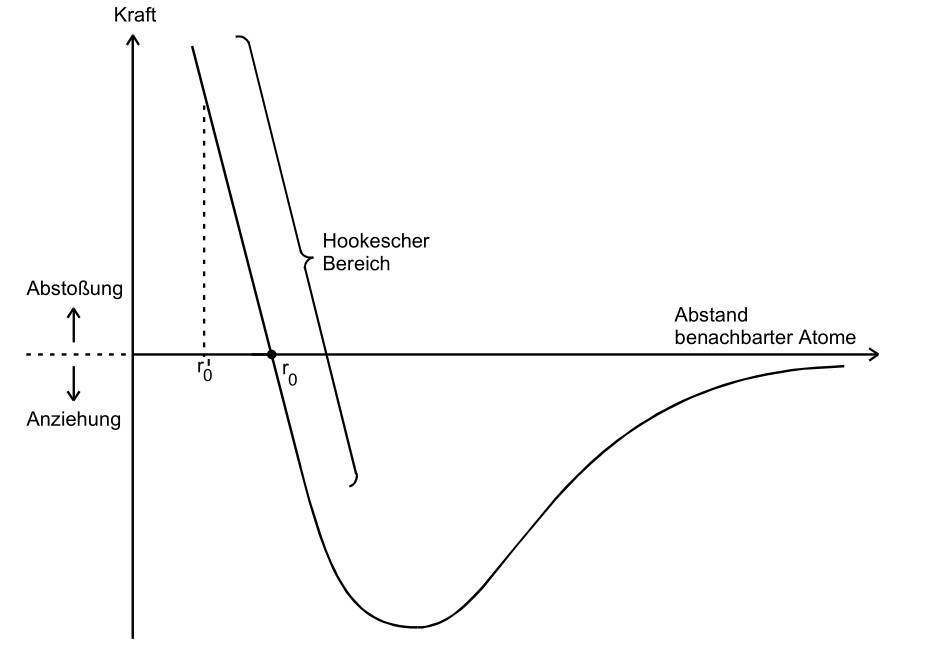
\includegraphics[width=0.8\textwidth]{bilder/kraftverlauf.jpg}
  \caption{Schematischer Kraftverlauf in einem Kristall\cite{102}}
  \label{kraft}
\end{figure}
Liegt $r\'_0$ in dem in Abbildung \ref{kraft} Bereich, ist der Vorgang
reversibel. Dies bedeutet, dass nach Verschwinden der äußeren Kraft $r\'_0$
wieder in $r_0$ über geht.

In einem Kristall benötigt es jeweils 6 Komponenten für die Beschreibung der
Spannung und der Deformation. Hierdurch entsteht eine 6x6-Matrix. Es sind sind
also 36 Komponenten nötig. Durch das Energieprinzip lässt sich diese Anzahl auf
21 reduzieren. Weitere elastische Konstanten lassen sich durch Symmetrien
eliminieren.
\subsection{Elastische Konstanten isotroper Stoffe}
Ein Körper mit richtungsunabhängigen elastischen Konstanten, also ein isotroper
Körper, soll in dem Experiment untersucht werden. Dafür werden zwei Konstanten
benötigt:
Das Schub- oder Torsionsmodell G für die Gestaltselastizität und den
Kompressionsmodul Q für die Volumenelastizität. Hinzu kommt der Elastizitätsmodul
E, welcher bereits in Gleichung \eqref{eq:hook} definiert wurde. Dieser ist für
die relative Längenänderung beim Angreifen einer Normalspannung in
Spannungsrichtung. Die Poissonsche Querkontraktionszahl $\mu$ steht für die
Längenänderung senkrecht zur Normalspannung und ist über
\begin{equation}
  \mu = -\frac{\Delta B}{B}\cdot\frac{L}{\Delta L}
  \label{eq:qkz}
\end{equation}
definiert. Abbildung \ref{qkz} erklärt die Querkontraktionszahl an einem
gedehnten Stab.
\begin{figure}[H]
  \centering
  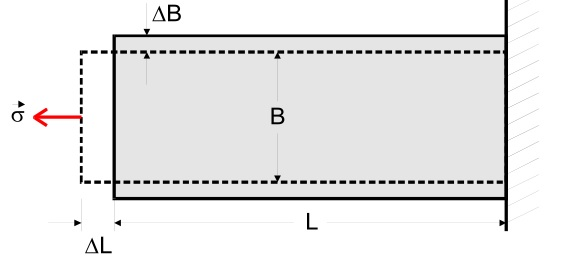
\includegraphics[width=0.8\textwidth]{bilder/kontraktionszahl.jpg}
  \caption{Erklärung der Querkontraktionszahl an einem gedehnten Stab \cite{102}
  }
  \label{qkz}
\end{figure}
Nach der Elastizitätstheorie gelten für isotrope Körper die Beziehungen
\begin{equation}
  E = 2 G (\mu+1)\leftrightarrow \mu=\frac{E}{2G}-1
\end{equation}
und
\begin{equation}
  E = 3(1-2\mu)Q\leftrightarrow Q=\frac{E}{3(1-2\mu)}.
\end{equation}
Welches sich vereinfacht als
\begin{equation}
  Q=\frac{EG}{9G-3E}
\end{equation}
schreiben lässt. Wenn für Proben $ L \gg B$ gilt, lassen sich das Elastizitäts-
und das Schubmodul leicht bestimmen.
\newpage
\subsection{Bestimmung des Schubmoduls G}
Treten bei einem Körper nur Tangentialspannungen auf, kommt es zu einer Scherung
. Der Körper wird dabei in eine Richtung deformiert. Da sich der Scherungswinkel
jedoch nur sehr ungenau bestimmen lässt, wird G häufig aus einer Torsion heraus
bestimmt.
\begin{figure}
  \centering
  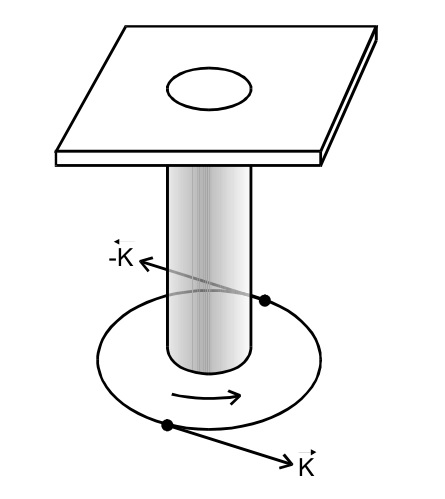
\includegraphics[height=0.5\textwidth]{bilder/torsion.jpg}
  \caption{Torsion am Zylinder}
  \label{torsion}
\end{figure}
Bei der Torsion wird der Körper an einem Ende festgespannt und lässt am anderen
Ende zwei diametral gegenüberliegende Punkten ein Kräftepaar wie in Abbildung
\ref{torsion} angreifen. Der Körper erfährt dann ein Drehmoment, welches eine
Verdrehung der unteren Fläche gegen die obere um den Winkel $\varphi$ hervorruft
. Abbildung \ref{drill} zeigt die Verdrillung einer zylindrischen Probe.
\begin{figure}[H]
  \centering
  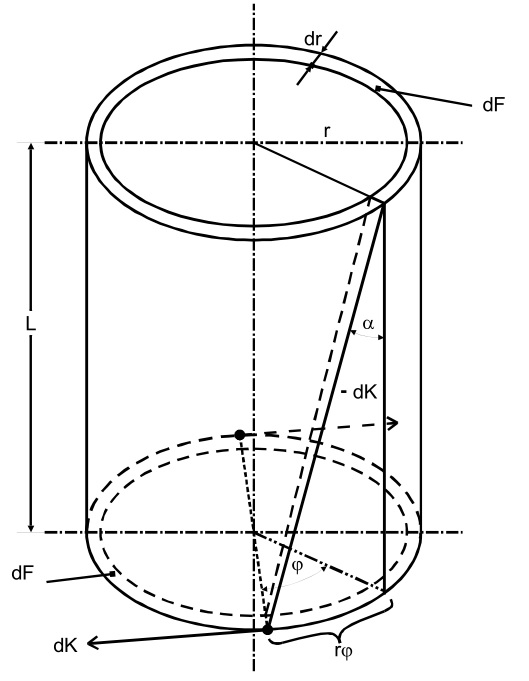
\includegraphics[height=0.5\textwidth]{bilder/verdrillung.jpg}
  \caption{Zusammenhang zwischen Drehmoment und Verdrillungswinkel am Zylinder
  \cite{102}}
  \label{drill}
\end{figure}
Das endgültige Drehmoment lässt sich über
\begin{equation}
  M=\int_0^\su{R} 2\pi\frac{G}{L}\varphi r^3\su{dr}=\frac{\pi}{2}G\frac{R^4}
  {L}\varphi
  \label{eq:drehmoment}
\end{equation}
berechnen. Der Proportionalitätsfaktor, oder Richtgröße, beträgt dann
\begin{equation}
  D:=\frac{\pi GR^4}{2L}
  \label{eq:richt}
\end{equation}
Die Problematik von elastischen Nachwirkungen wird durch ein Messverfahren
vermieden, bei welcher die Spannung eine periodische Funktion der Zeit ist.
Für dieses Messverfahren wird eine Kugel an den Draht gehangen und ausgelenkt.
Durch die Torsion des Drahtes kommt es zu entgegengesetzt wirkenden Drehmomenten
Somit entsteht eine Differentialgleichung zweiter Ordnung, welche durch den
Cosinussatz
\begin{equation}
  \varphi(t)=\varphi_0\cos\frac{2\pi}{T}t
\end{equation}
gelöst wird. Für die Periodendauer T ergibt sich dann die Beziehung
\begin{equation}
  T=2\pi\sqrt{\frac{\Theta}{D}}.
  \label{eq:period}
\end{equation}
Wobei $\Theta$ das Trägheitsmoment der Kugel ist und D die Richtgröße.
Das Gesamtträgheitsmoment der Kugel ergibt sich durch die Gleichung
\begin{equation}
  \Theta_\su{K}=\frac{2}{5} m_\su{k}R_\su{k}^2
  \label{eq:theta}
\end{equation}
Aus den Formeln \eqref{eq:richt},\eqref{eq:period} und \eqref{eq:theta} ergibt sich
eine endgültige Gleichung für die Berechnung des Schubmoduls:
\begin{equation}
  G= \frac{16}{5}\pi\frac{m_\su{k}R_\su{k}^2L}{T^2R^4}
\end{equation}
\subsection{Magnetisches Moment des Permanentmagneten}
Um das magnetische Moment zu messen, sei
\begin{equation}
  \vec{m}:=p\vec{a}
\end{equation}
gegeben. Hierbei ist p die Polstärke und $\vec{a}$ der Abstand der Pole. Ist das
Magnetfeld homogen, wirken aufgrund des unterschiedlichen Vorzeichens von p zwei
entgegengesetzte Kräfte auf den Magneten, wie in Abbildung \ref{magnet} zu sehen.
\begin{figure}[H]
  \centering
  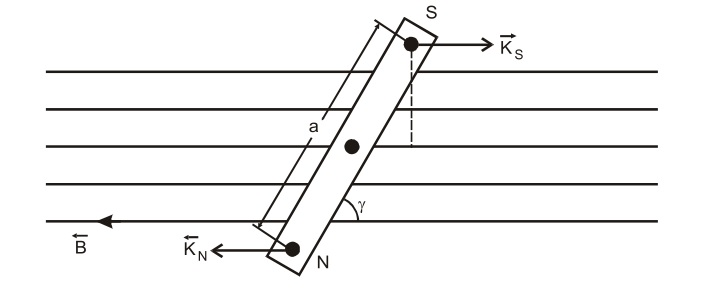
\includegraphics[width=0.8\textwidth]{bilder/magnet.jpg}
  \caption{Permanentmagnet in einem äußeren Magnetfeld \cite{102}}
  \label{magnet}
\end{figure}
Es wirkt ein Magnetfeld, welches durch
\begin{equation}
  M_\su{Mag}=mB\sin(\gamma)
\end{equation}
charakterisiert ist. Die nicht-lineare Differentialgleichung wird durch
Kleunwinkelnäherung linearisiert und lässt sich durch einen Cosinussatz lösen.
Für die Periodendauer ergibt sich dann:
\begin{equation}
  T_\su{m}=2\pi\sqrt{\frac{\Theta}{mB+D}}
  \label{eq:magperi}
\end{equation}
